%%%%%%%%%%%%%%%%%%%%%%%%%%%%%%%%%%%%%%%%%%%%%%%%%%%%%%%%%%%%%%%%%%%%%%%%%%%%%%%%%%
\begin{frame}[fragile]\frametitle{}
\begin{center}
{\Large Concepts}
\end{center}
\end{frame}

%%%%%%%%%%%%%%%%%%%%%%%%%%%%%%%%%%%%%%%%%%%%%%%%%%%%%%%%%%%%%%%%%%%%%%%%%%%%%%%%%%
\begin{frame}[fragile]\frametitle{Example}


\begin{itemize}
\item A robot looks at boxes on a conveyor belt and segregates them into Good or Bad bins based on their weight.
\item What's the Environment, Action, Agent and Reward here?

\end{itemize}

\begin{center}
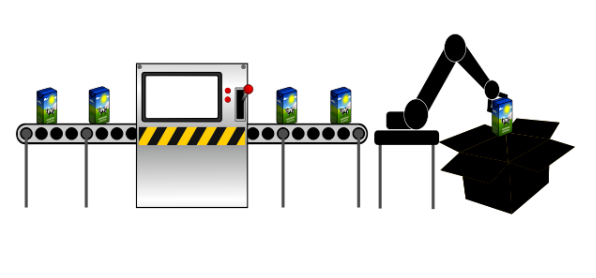
\includegraphics[width=0.8\linewidth,keepaspectratio]{rl68}
\end{center}

{\tiny (Ref: Modern Reinforcement Learning: Deep Q Learning in PyTorch - Phil Tabor)}

\end{frame}

%%%%%%%%%%%%%%%%%%%%%%%%%%%%%%%%%%%%%%%%%%%%%%%%%%%%%%%%%%%%%%%%%%%%%%%%%%%%%%%%%%
\begin{frame}[fragile]\frametitle{Core Concepts in the Example}


\begin{itemize}
\item Agent is whoever acts: Robot's memory of (states, actions, rewards)
\item Environment: What changes when Agent (Robot) acts upon? : Boxes. Position of the boxes change and Rewards given to the agent/robot. So, Environment = Boxes + Rewards. Btw, Rewards are always with Environment.
\item Reward, indicator that heps decision: Good/Bad
\item State: Reading on the weight sensor.State space is the range of weights possible.
\item Action: Discrete (move to good/bad bin), causes new box to load, then new weight happens. Q Learning works on Discrete spaces like this but for continuous spaces algorithms like Actor-Critique are used.
\end{itemize}

\begin{center}
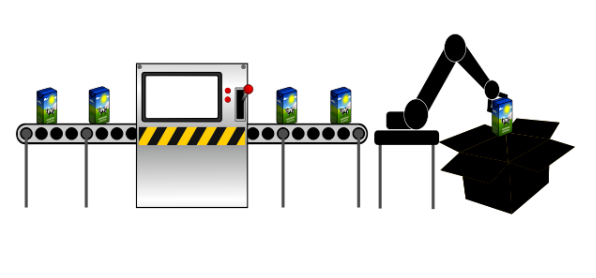
\includegraphics[width=0.4\linewidth,keepaspectratio]{rl68}
\end{center}

{\tiny (Ref: Modern Reinforcement Learning: Deep Q Learning in PyTorch - Phil Tabor)}

\end{frame}

%%%%%%%%%%%%%%%%%%%%%%%%%%%%%%%%%%%%%%%%%%%%%%%%%%%%%%%%%%%%%%%%%%%%%%%%%%%%%%%%%%
\begin{frame}[fragile]\frametitle{Environment}


\begin{center}
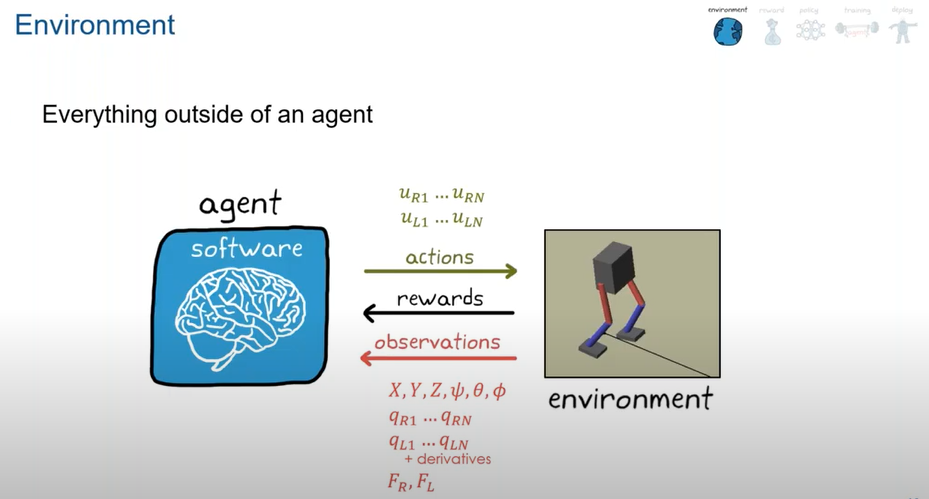
\includegraphics[width=0.9\linewidth,keepaspectratio]{rl76}
\end{center}

{\tiny (Ref: How to Train Your Robot: An Introduction to Reinforcement Learning - Craig Buhr PhD)}

\end{frame}

%%%%%%%%%%%%%%%%%%%%%%%%%%%%%%%%%%%%%%%%%%%%%%%%%%%%%%%%%%%%%%%%%%%%%%%%%%%%%%%%%%
\begin{frame}[fragile]\frametitle{Real vs Simulated Environment}


\begin{center}
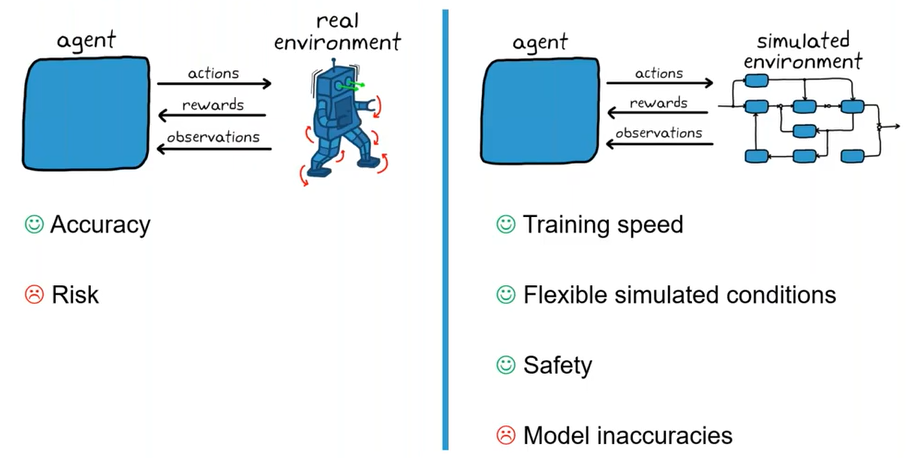
\includegraphics[width=0.9\linewidth,keepaspectratio]{rl77}
\end{center}

{\tiny (Ref: How to Train Your Robot: An Introduction to Reinforcement Learning - Craig Buhr PhD)}

\end{frame}

%%%%%%%%%%%%%%%%%%%%%%%%%%%%%%%%%%%%%%%%%%%%%%%%%%%%%%%%%%%%%%%%%%%%%%%%%%%%%%%%%%
\begin{frame}[fragile]\frametitle{Reward}


\begin{center}
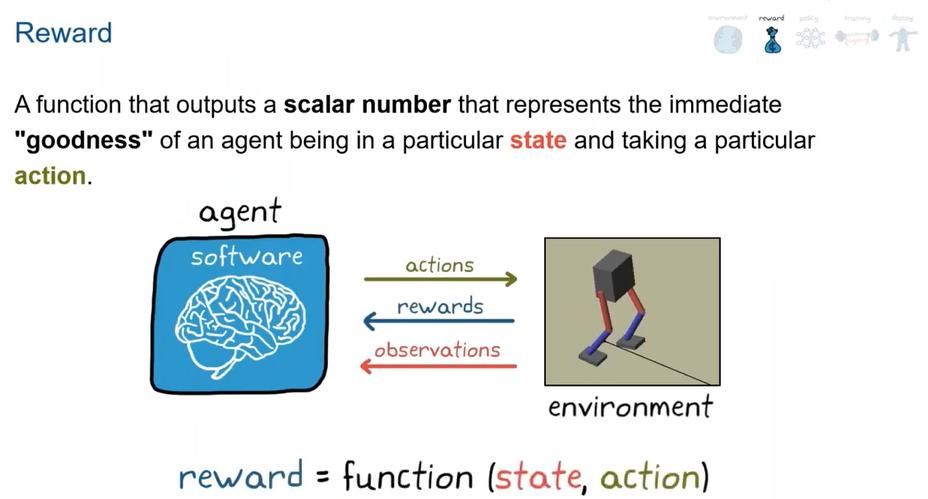
\includegraphics[width=0.9\linewidth,keepaspectratio]{rl78}
\end{center}

{\tiny (Ref: How to Train Your Robot: An Introduction to Reinforcement Learning - Craig Buhr PhD)}

\end{frame}

%%%%%%%%%%%%%%%%%%%%%%%%%%%%%%%%%%%%%%%%%%%%%%%%%%%%%%%%%%%%%%%%%%%%%%%%%%%%%%%%%%
\begin{frame}[fragile]\frametitle{Defining Reward}

For Robot walking in straight line, it should not fall, be fast, etc.

\begin{center}
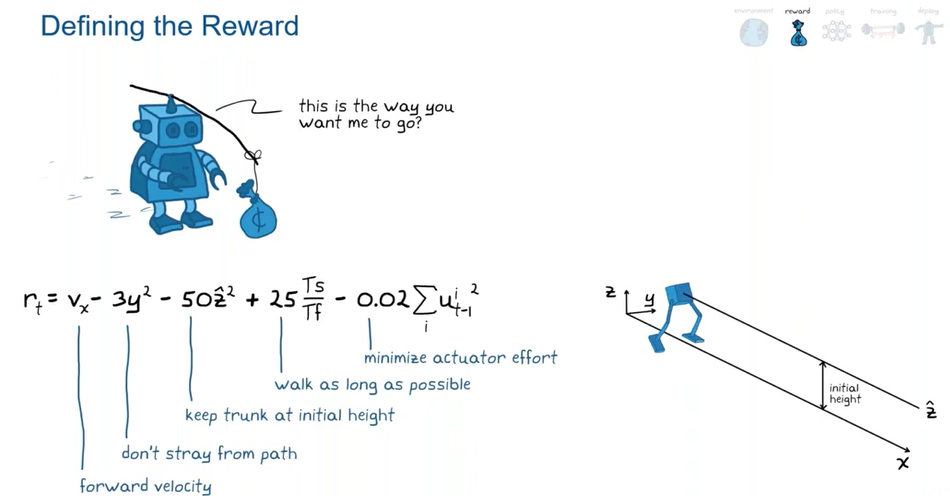
\includegraphics[width=0.9\linewidth,keepaspectratio]{rl79}
\end{center}

{\tiny (Ref: How to Train Your Robot: An Introduction to Reinforcement Learning - Craig Buhr PhD)}

\end{frame}

%%%%%%%%%%%%%%%%%%%%%%%%%%%%%%%%%%%%%%%%%%%%%%%%%%%%%%%%%%%%%%%%%%%%%%%%%%%%%%%%%%
\begin{frame}[fragile]\frametitle{Policy: Actor Critic Method}


\begin{center}
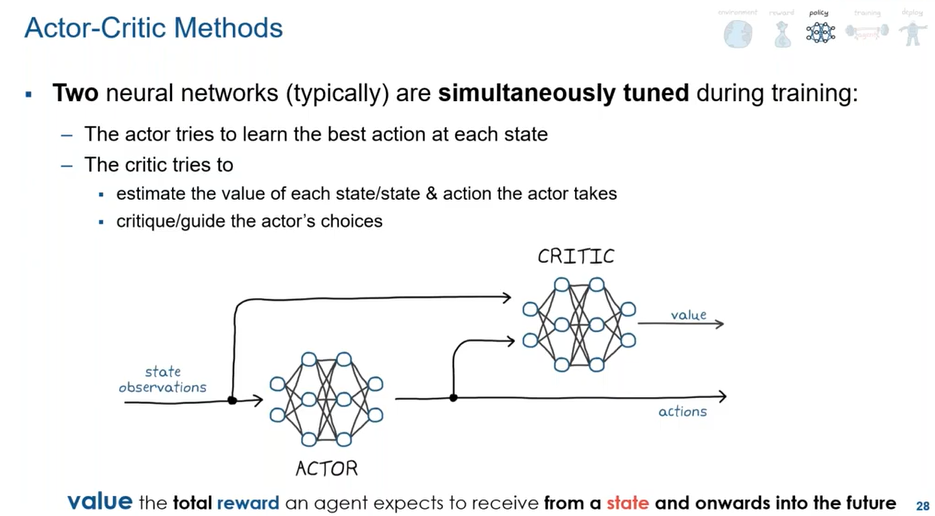
\includegraphics[width=0.9\linewidth,keepaspectratio]{rl80}
\end{center}

{\tiny (Ref: How to Train Your Robot: An Introduction to Reinforcement Learning - Craig Buhr PhD)}

\end{frame}

%%%%%%%%%%%%%%%%%%%%%%%%%%%%%%%%%%%%%%%%%%%%%%%%%%%%%%%%%%%%%%%%%%%%%%%%%%%%%%%%%%
\begin{frame}[fragile]\frametitle{Training: Actor Critic Method}


\begin{center}
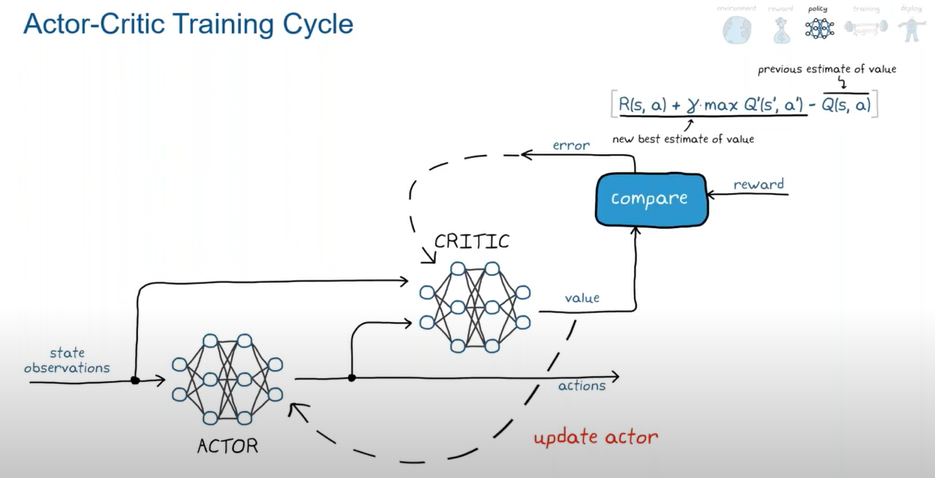
\includegraphics[width=0.9\linewidth,keepaspectratio]{rl81}
\end{center}

{\tiny (Ref: How to Train Your Robot: An Introduction to Reinforcement Learning - Craig Buhr PhD)}

\end{frame}


%%%%%%%%%%%%%%%%%%%%%%%%%%%%%%%%%%%%%%%%%%%%%%%%%%%%%%%%%%%%%%%%%%%%%%%%%%%%%%%%%%
\begin{frame}[fragile]\frametitle{Core Concepts by Definition}


\begin{itemize}
\item Agent : Entity learning about the environment and making decisions. We need to specify a learning algorithm for the agent that allows it to learn a policy
\item Environment: Everything outside the agent, including other agents
\item Rewards: Numerical quantities that represent feedback from the environment that an agent tries to maximize
\item State: A representation of the environment. At time step $t$,the agent is in state $S_t \in S$ where $S$ is the set of all possible states
\item Action: At time step $t$, an agent takes an action $A_t \in A(S_t)$ where $A(S_t)$ is the set of actions available in state $S_t$
\item Policy: A policy tells the agent what action to take in a given state $\pi(a|S)$. A policy can be deterministic i.e. there is one action that is deterministically selected in a given state $\pi(s)=a$, or stochastic i.e. the policy maps a state onto a set of probabilities for taking each action. $p(a_i|s) < 1$ subject to $\sum_{i} p(a_i|s) = 1$
\item To solve a problem using RL, we should be able to formulate it as a Markov Decision Process (MDP).
\end{itemize}



{\tiny (Ref: Solving Tic-Tac-Toe with Reinforcement Learning - Govind G Nair)}

\end{frame}

%%%%%%%%%%%%%%%%%%%%%%%%%%%%%%%%%%%%%%%%%%%%%%%%%%%%%%%%%%%%%%%%%%%%%%%%%%%%%%%%%%
\begin{frame}[fragile]\frametitle{Core Concepts by Definition}


\begin{itemize}
\item In an MDP, the environment is completely characterized by the transition dynamics equation $p(s',r|s,a)$.
\item That is, the probability of each possible value for $s'$ (the subsequent state) and $r$ (reward) depends only on the immediately preceding state and action,$s$ and $a$, and, given them, not at all on earlier states and actions. In other words, given the present, the future is independent of the past.
\item The state must include information about all aspects of the past agent–environment interaction that make a difference for the future. If it does, then the state is said to have the Markov property
\item If the transition dynamics equation is fully known by the agent, it means an optimal policy can be computed without interacting with the environment. This is planning. Some kind of search algorithm can be used here.
\item When the environment is not fully known, the agent has to learn by interacting with the environment. i.e. learning. If an agent constructs a model of the environment , it is called model based RL, else it is called model free RL.
\end{itemize}



{\tiny (Ref: Solving Tic-Tac-Toe with Reinforcement Learning - Govind G Nair)}

\end{frame}

%%%%%%%%%%%%%%%%%%%%%%%%%%%%%%%%%%%%%%%%%%%%%%%%%%%%%%%%%%%%%%%%%%%%%%%%%%%%%%%%%%
\begin{frame}[fragile]\frametitle{Core Concepts by Definition}


\begin{itemize}
\item When an agent in state $s_t$ takes an action $A_t$ as prescribed by a policy $\pi$ , it transitions to a state $s_{t+1}$ and receives a reward $R_{t+1}$. The Agent interacting with the ``MDP'' environment thus gives rise to a sequence or trajectory $S_0,A_0,R_1,S_1,A_1,R_2,S_2,\ldots$
\item The goal of an agent is to maximize the long term reward or return.
\item Long term reward or return is formally defined as the discounted sum of future rewards. $G_t = R_{t+1} + \gamma R_{t+2} + \gamma R_{t+3} + \ldots = \sum_{k=0}^{\infty} \gamma^k R{t+k+1} = R_{t+1} + \gamma G_{t+1}$
\end{itemize}



{\tiny (Ref: Solving Tic-Tac-Toe with Reinforcement Learning - Govind G Nair)}

\end{frame}


%%%%%%%%%%%%%%%%%%%%%%%%%%%%%%%%%%%%%%%%%%%%%%%%%%%%%%%%%%%%%%%%%%%%%%%%%%%%%%%%%%
\begin{frame}[fragile]\frametitle{Core Concepts}


\begin{itemize}
\item 3 main components of RL: Q function, Policy function, model function
\item As deep learning can approximate any function over large state space it has become good representation learning for all 3 components. For small state space tables are ok but for large problems and continuous states like football field, function approximation is needed
\item How to evaluate a position? Let it play from there randomly till end with multiple ways, average them and that's the value. Monte Carlo tree search. Limited success.
\item Alpha go was with deep learning and not search

\end{itemize}

\end{frame}

%%%%%%%%%%%%%%%%%%%%%%%%%%%%%%%%%%%%%%%%%%%%%%%%%%%%%%%%%%%%%%%%%%%%%%%%%%%%%%%%%%
\begin{frame}[fragile]\frametitle{Observations vs States}

\begin{itemize}
\item Observation and State are different. Pixels of image are observation. State is what is there. Image is what is seen now. Observations result from state. Its like a view of underlying data.
\item Past observations give you additional information. But for states, being true, the last one is good enough.
\end{itemize}


\begin{center}
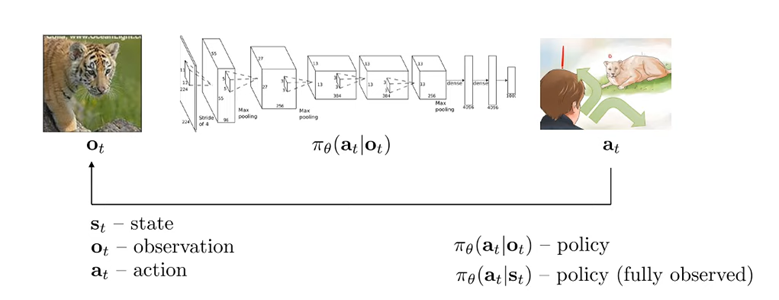
\includegraphics[width=0.8\linewidth,keepaspectratio]{rl48}
\end{center}


{\tiny (Ref: CS 285 Fall 2020 Deep Reinforcement Learning)}

\end{frame}

%%%%%%%%%%%%%%%%%%%%%%%%%%%%%%%%%%%%%%%%%%%%%%%%%%%%%%%%%%%%%%%%%%%%%%%%%%%%%%%%%%
\begin{frame}[fragile]\frametitle{How to learn Policy?}


\begin{center}
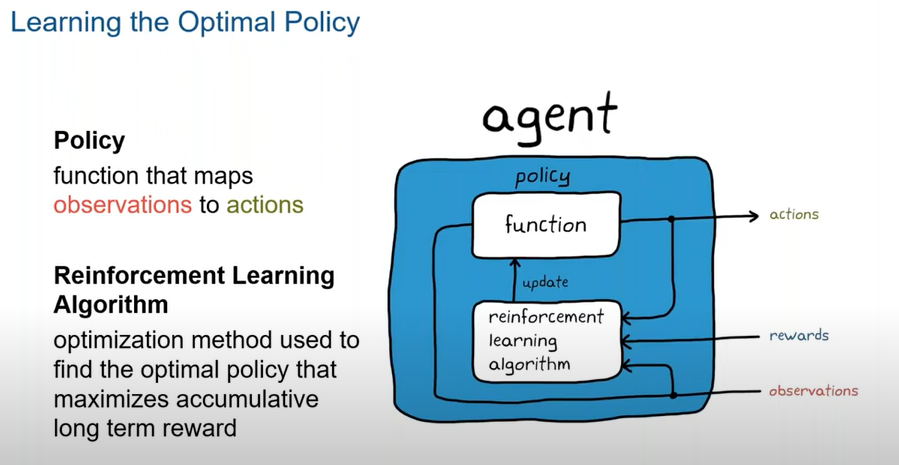
\includegraphics[width=0.9\linewidth,keepaspectratio]{rl75}
\end{center}

{\tiny (Ref: How to Train Your Robot: An Introduction to Reinforcement Learning - Craig Buhr PhD)}

\end{frame}


%%%%%%%%%%%%%%%%%%%%%%%%%%%%%%%%%%%%%%%%%%%%%%%%%%%%%%%%%%%%%%%%%%%%%%%%%%%%%%%%%%
\begin{frame}[fragile]\frametitle{How to learn Policy?}

Imitation Learning (behavior cloning): Take labelled data and do supervised learning. It does not work as a small mistake can amplify later. But with good data from additional cameras, it can correct the path.


\begin{center}
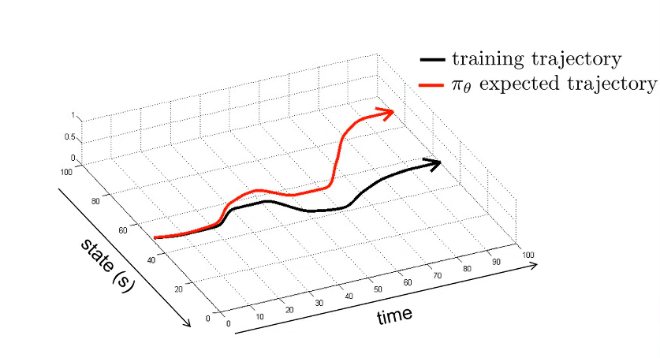
\includegraphics[width=0.4\linewidth,keepaspectratio]{rl49}

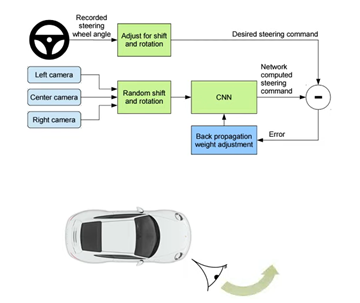
\includegraphics[width=0.4\linewidth,keepaspectratio]{rl50}

\end{center}

Markovian means if we see the same thing twice, we do the same thing twice, regardless of what happened before.


{\tiny (Ref: CS 285 Fall 2020 Deep Reinforcement Learning)}

\end{frame}


%%%%%%%%%%%%%%%%%%%%%%%%%%%%%%%%%%%%%%%%%%%%%%%%%%%%%%%%%%%%%%%%%%%%%%%%%%%%%%%%%%
\begin{frame}[fragile]\frametitle{Observations vs States}

\begin{itemize}
\item If you have observations, then past observations would be needed to find the truth (state), but if you have ready states then just the past/current one is good enough to decide the future action.
\item If predictions and data diverge, how to converge them? DAagger: Dataset Aggregation. Get data from predictions only. First train on human data, then run to predict, then have humans label the predictions/actions. Merge both datasets. Train on the whole dataset. Repeat to converge.
Conditions when Fit-the-expert strategy fails:
\begin{itemize}
\item Non-Markovian behavior: action depends not only on the past state but more. At same state actions are different.
\item 	Multimodal behavior: different streams of inputs decide the action.
\end{itemize}

\end{itemize}


\begin{center}
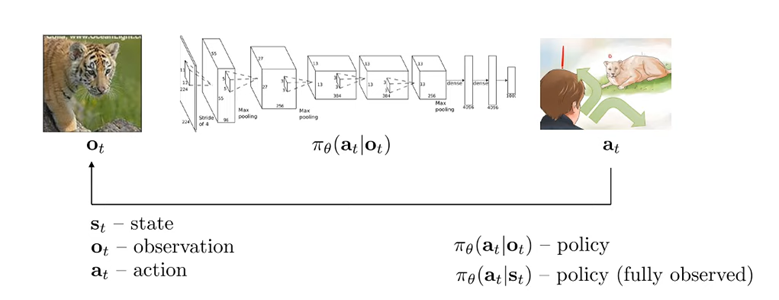
\includegraphics[width=0.8\linewidth,keepaspectratio]{rl48}
\end{center}


{\tiny (Ref: CS 285 Fall 2020 Deep Reinforcement Learning)}

\end{frame}